\section{Visualization}
\label{sec:KSeMF}

To visualize the reduced \statesp\ of KS flow we will use a
moving frame to compute the first few fundamental invariants
of the action of $\SOn{2}$ and, following the example of
\CLe\ of \refsect{sec:CLeMF}, modify these invariants to
overcome these singularities. This will help us understand
what the invariant objects of importance in organizing the
\statesp\ are. The final goal is to choose Poincar\'e
sections that capture the dynamics but on which we can define
local {\csection}s, implement symmetry reduction on the
Poincar\'e sections applying a moving frame on the points of
intersection of trajectories with the Poincar\'e sections and
finally construct return maps of the dynamics. At
this point we do not quotient out the discrete symmetry. This
can always do afterwards by utilizing a fundamental domain,
as in \refchap{chap:Lorenz}.


We begin by computing invariants for the ``standard action''
\refeq{eq:SO2stndrd} of $\SOn{2}$ on $\Clx{N}\cong\Rls{2N}$
which we write here as
\beq
	\left(\barr{cc} \overline{b}_k \\ \overline{c}_k\earr \right)=\left(\barr{cc}
			    			\cos(k\theta) & -\sin(k\theta)\\
						\sin(k\theta) & \cos(k\theta)\\
			   			\earr	
						\right) \left(\barr{cc} b_k \\ c_k\earr\right)\,,\ \ k=1,\ldots N\,.
	\label{eq:SO2stand}
\eeq
with $a_k=b_k+i c_k\,,\ b_k,c_k\in\Rls{}$.
The choice of a {\csection} is arbitrary and thus, after some
experimentation, we choose one that results in convenient
algebra.
Define the {\csection} by
\beq
 	K_1(a)=c_1=0\,,\qquad b_1>0\,
\eeq
which leads to the normalization equation
\beq
	\overline{c}_1 = \sin\theta\, b_1 +\cos\theta\, c_1 = 0\,.
	\label{eq:SO2norm}
\eeq
from which we obtain the moving frame
\beq
	\theta=-\tan^{-1}\frac{c_1}{b_1}\,,
	\label{eq:SO2stand1}
\eeq
where, as noted in \refchap{chap:lasers}, $\tan^{-1}$
distinguishes quadrants. Substituting the moving frame into
the rest of \refeq{eq:SO2stand} we get the fundamental
invariants for the action of $\SOn{2}$ in Fourier space of
\KS\ equation. The simplifications of expressions were
performed using computer algebra system Mathematica.
Computation of $255$ invariants for $n=128$ took
approximately $20$ minutes on a typical processor. We list
the first $11$ invariants on \reftab{tab:SO2n6}. It is
important to note that computation in each irreducible
subspace (for each $k$ in \refeq{eq:SO2stand}) can be carried
out independently and thus we can parallelize the
computations and also avoid recomputing invariants when
increasing $N$. For the present visualization purposes,
though, the  invariants listed in \reftab{tab:SO2n6} are more
than enough.


\begin{table}[t]
\caption[Fundamental invariants for standard action of $\SOn{2}$]
{First $11$ fundamental invariants for the standard action
 \refeq{eq:SO2stand} of \SOn{2} on \Rls{2N}.}
\scriptsize
\[
\begin{array}{ll}
  u_1=r_1=\sqrt{b_1^2+c_1^2}&  \\ u_3=\frac{b_2 \left(b_1^2-c_1^2\right)+2 b_1 c_1 c_2}{r_1^2}&u_4=\frac{-2
b_1 b_2 c_1+\left(b_1^2-c_1^2\right) c_2}{r_1^2}\\ u_5=\frac{b_1 b_3 \left(b_1^2-3 c_1^2\right)-c_1 \left(-3
b_1^2+c_1^2\right) c_3}{r_1^3}&u_6=\frac{-3 b_1^2 b_3 c_1+b_3 c_1^3+b_1^3 c_3-3 b_1 c_1^2 c_3}{r_1^3}\\ u_7=\frac{b_4
\left(b_1^4-6 b_1^2 c_1^2+c_1^4\right)+4 b_1 c_1 \left(b_1^2-c_1^2\right) c_4}{r_1^4}&u_8=\frac{4 b_1
b_4 c_1 \left(-b_1^2+c_1^2\right)+\left(b_1^4-6 b_1^2 c_1^2+c_1^4\right) c_4}{r_1^4}\\ u_9=\frac{b_1
b_5 \left(b_1^4-10 b_1^2 c_1^2+5 c_1^4\right)+c_1 \left(5 b_1^4-10 b_1^2 c_1^2+c_1^4\right) c_5}{r_1^5}&u_{10}=\frac{-b_5
c_1 \left(5 b_1^4-10 b_1^2 c_1^2+c_1^4\right)+b_1 \left(b_1^4-10 b_1^2 c_1^2+5 c_1^4\right) c_5}{r_1^5}\\ u_{11}=\frac{b_6
\left(b_1^6-15 b_1^4 c_1^2+15 b_1^2 c_1^4-c_1^6\right)+2 b_1 c_1 \left(3 b_1^4-10 b_1^2 c_1^2+3 c_1^4\right) c_6}{r_1^6}&u_{12}=\frac{-2
b_1 b_6 c_1 \left(3 b_1^4-10 b_1^2 c_1^2+3 c_1^4\right)+\left(b_1^6-15 b_1^4 c_1^2+15 b_1^2 c_1^4-c_1^6\right) c_6}{r_1^6}\\
\end{array}
\]
\label{tab:SO2n6}
\end{table}

As was the case in \CLe\ example in \refchap{chap:lasers},
there is an obvious singularity at $b_1=c_1=0$ that can be corrected by substituting
$r_1$ with
$r=\sum_{i=1}^N (b_i^2+c_i^2)$ in the denominators.
Here we will instead use \ESedit{$r=\sqrt{\sum_{i=1}^3 (b_i^2+c_i^2)}$}
since
dynamics in our case like to visit $\EQV{2}$ and $\EQV{3}$
and this choice is enough to prevent the denominator from
vanishing at any region of \statesp\ of dynamical interest.
Even with this modification one has to note that problems
are still present: the invariants of
\reftab{tab:SO2n6} vanish at \EQB{2} and \EQB{3} (in general
they vanish on $b_1=c_1=0$).
%ES dropped: In principle
% this is not a problem since we want to carry out reduction in
% the principal stratum. In practice
This causes two important
\eqva\ to be mapped to the origin and leads to \statesp\
portraits as in \reffig{fig:ksSO2eqbTo0}. The neighborhood of
\EQB{2} and \EQB{3} which is where we would like to get some
intuition about the behavior of \rpo s, has been squeezed into
a kink shaped structure.
Inspection of the invariants in \reftab{tab:SO2n6} reveals
that the problem is caused by $b_1$ and $c_1$ (which vanish
at \EQV{2}, \EQV{3}) appearing in all monomials in the
numerators. This is related to the fact that we have chosen
the {\csection} in the $k=1$-irreducible subspace which
introduces $b_1$ and $c_1$ through the substitution of
\refeq{eq:SO2stand} into \refeq{eq:SO2norm}. Note that the
{\csection} does not exist when $b_1=c_1=0$, as there the
group action fails to be regular when restricted on the
$k=1$-irreducible subspace.
\PCedit{
We still lack group-theoretical understanding
of this behavior.
}
We could overcome this
difficulty by using the second, third, or sixth Fourier mode
to setup the moving frame but then the expressions we get
after substitution cannot be fully simplified and we loose
the ability to manipulate the denominators. We will use a
higher mode to setup the moving frame in the numerical
implementation, though, after we define suitable Poincar\'e
sections, see \refchap{chap:tobedone}.

%%%%%%%%%%%%%%%%%%%%%%%%%%%%%%%%%%%%%%%%%%%%%%%%%%%%%%%%%%%%%%%%%%
\begin{figure}[t]
\begin{center}
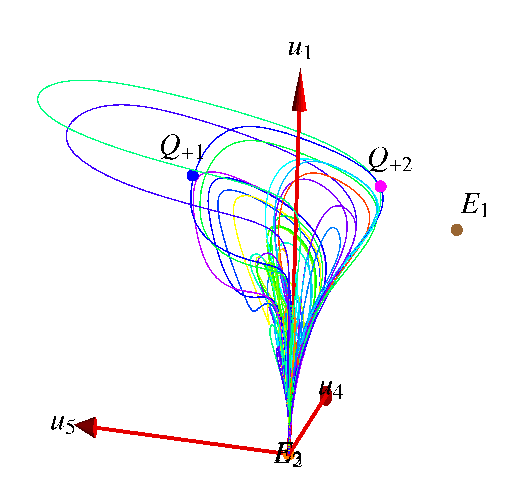
\includegraphics[width=0.4\textwidth, clip=true]{../figs/ksSO2inv145eqbTo0}
\end{center}
\caption[\KS\ \SOn{2} reduced \statesp, modified invariants]
   {\Statesp\ portrait of $L=22$ \KS\ dynamics projected to
   invariants given in \reftab{tab:SO2n6}. The trajectories
   shown are 20 short \rpo s. }
\label{fig:ksSO2eqbTo0}
\end{figure}
%%%%%%%%%%%%%%%%%%%%%%%%%%%%%%%%%%%%%%%%%%%%%%%%%%%%%%%%%%%%%%%%

For visualization purposes we overcome the problem by modifying
the invariants of \reftab{tab:SO2n6} as follows. We observe
that the invariants come as either symmetric or antisymmetric
under the action of $\Dn{1}\subset\On{2}$. We modify the
symmetric invariants by adding a term $\sqrt{b_i^2+c_i^2}$
where $i$ labels the corresponding irreducible subspace  (Fourier
mode). The new invariants are listed in
\reftab{tab:SO2n6modif}.
\RLD{Since $r$ is defined as the sum of squares, I think that $r_1$ in the denominator should be replaced with $r^{1/2}$.  So, it should be $r$ instead of $r^2$ in $u_3$ and $u_4$, $r^{3/2}$ instead of $r^3$ in $u_5$ and $u_6$, etc. {\bf ES}: Thanks! There was a typo in definition of $r$. A square root should be there.}
One has to note that such a modification is not unique as any
linear combination of invariants is an invariant. The basic
requirement is that the invariants remain linearly
independent, which can be easily verified for the present
choice. The motivation behind this choice, apart from its
simplicity (the magnitudes of Fourier modes are \SOn{2}-invariant) is
that if we set up a {\csection} by $c_i=0$ then the
invariant that we get associated with the $i$'th irreducible
subspace is $\sqrt{b_i^2+c_i^2}=0$ (and the trivial invariant
$0$). A linear combination of invariants resulting from more
than one moving frame is a natural choice since the problem
is caused by only taking into account the $i=1$-mode in
setting up the moving frame. Computing a full set of
invariants using a moving frame in every irreducible subspace
would be time consuming. For the group action we examine here
the algebra required to obtain explicit expressions was not
carried out
%\PCedit dropped this: by Mathematica
and thus we only use the simplest available invariants, the
Fourier magnitudes. An other choice would be to replace the
$\Dn{1}$-invariant by the \ESedit{Fourier} magnitudes instead of forming a
linear combination, but we have found that the resulting
phase space portraits are not as useful.


\begin{table}
\caption[Modified invariants for $\SOn{2}, n=6$]
{Modified invariants for the standard action of \SOn{2} on \Rls{6}}
\label{tab:SO2n6modif}
\begin{small}
\begin{eqnarray*}
  u_1=r_1 &=&\sqrt{b_1^2+c_1^2}\\
  u_3 &=&\frac{b_2 \left(b_1^2-c_1^2\right)+2 b_1 c_1 c_2}{r^2}\\
  u_4 &=&\sqrt{b_2^2+c_2^2}+\frac{-2
b_1 b_2 c_1+\left(b_1^2-c_1^2\right) c_2}{r^2}\\
  u_5 &=&\sqrt{b_3^2+c_3^2}+\frac{b_1 b_3 \left(b_1^2-3 c_1^2\right)-c_1 \left(-3
b_1^2+c_1^2\right) c_3}{r^3}\\
  u_6 &=&\frac{-3 b_1^2 b_3 c_1+b_3 c_1^3+b_1^3 c_3-3 b_1 c_1^2 c_3}{r^3}\\
  u_7 &=&\frac{b_4
\left(b_1^4-6 b_1^2 c_1^2+c_1^4\right)+4 b_1 c_1 \left(b_1^2-c_1^2\right) c_4}{r^4}\\
  u_8 &=&\sqrt{b_4^2+c_4^2}+\frac{4 b_1
b_4 c_1 \left(-b_1^2+c_1^2\right)+\left(b_1^4-6 b_1^2 c_1^2+c_1^4\right) c_4}{r^4}\\
  u_9 &=&\sqrt{b_5^2+c_5^2}+\frac{b_1
b_5 \left(b_1^4-10 b_1^2 c_1^2+5 c_1^4\right)+c_1 \left(5 b_1^4-10 b_1^2 c_1^2+c_1^4\right) c_5}{r^5}\\
  u_{10} &=&\frac{-b_5
c_1 \left(5 b_1^4-10 b_1^2 c_1^2+c_1^4\right)+b_1 \left(b_1^4-10 b_1^2 c_1^2+5 c_1^4\right) c_5}{r^5}\\
  u_{11} &=&\frac{b_6
\left(b_1^6-15 b_1^4 c_1^2+15 b_1^2 c_1^4-c_1^6\right)+2 b_1 c_1 \left(3 b_1^4-10 b_1^2 c_1^2+3 c_1^4\right) c_6}{r^6} \\
  u_{12} &=&\sqrt{b_6^2+c_6^2}+\frac{-2
b_1 b_6 c_1 \left(3 b_1^4-10 b_1^2 c_1^2+3 c_1^4\right)+\left(b_1^6-15 b_1^4 c_1^2+15 b_1^2 c_1^4-c_1^6\right) c_6}{r^6}
\end{eqnarray*}
\end{small}
\end{table}

\Statesp\ projections on the invariants of \reftab{tab:SO2n6modif} are shown in
\reffigTofig{fig:TW1red}{fig:TW1-E2red}.
Visualizing the unstable manifold of $\REQV{\pm}{1}$ is not a
straightforward task, since it is $4$-dimensional, see \reftab{tab:Eksym}.
Nevertheless, we observe that the ratio of real parts of the leading stability eigenvalues for the case of \REQV{\pm}{1} is approximately $3.4$ and thus we expect that the continuation of the strongly
unstable eigenspace will play the dominant role. Thus we can get an idea of the importance
of the unstable manifold of \REQV{\pm}{1} for the dynamics
by plotting the continuation of the $\eigExp[1,2]$ eigenplane under the flow,
until just after it appears to fold back to itself.
The way
in which sample {\rpo s} follow the unstable manifold in
\reffig{fig:TW1red} for some time before they visit different
regions of state space reveals the importance of this object
in organizing the flow, even though the immediate neighborhood of
\REQV{\pm}{1} is not visited by the ``turbulent'' dynamics or
the \rpo s.
At this time these observations are
of a rather speculative character as projections
are frequently misleading,
for instance the \rpo\ labeled $T=40.14$ in
\reffig{fig:TW1red} is not tracking the unstable manifolds as
well as implied by the figures, a fact that can be seen in
different projections. One could observe this already in
\reffig{fig:TW1red}, as the velocity on \rpo\ $T=40.14$ is
not aligned with the velocity of trajectories on the
manifold. In order to be able to decide whether a \rpo\ is
really influenced by an unstable manifold we need a notion of
distance of the two objects. This distance will be easier to measure
once we reduce the dynamics to discrete time maps on
suitable Poincar\'e sections, see \refchap{chap:tobedone}.

In \reffigpart{fig:TW1-E2red}{b} we can see that the parts of
the {\rpo s} that do not follow the unstable manifold of
\REQB{1} are ``captured'' by the unstable manifold of
\EQB{2}. One has to remember that this manifold is restricted
in the antisymmetric subspace while the {\rpo s} live in the
full space (more accurately, in the principal stratum).
Nevertheless the invariant objects in the antisymmetric
subspace provide a boundary for those orbits, in the same
 sense, that the $z$-axis in Lorenz flow
 of \refchap{chap:Lorenz} acts as a topological
obstruction to the flow. This behavior illustrates our point
of view that the dynamics can be described through maps
between a set of Poincar\'e sections, each associated with a
(relative) equilibrium and parameterized by intrinsic
coordinates such as the length along its unstable manifold.
Further pursuing this goal will be subject of future work,
see \refchap{chap:tobedone}.

It is interesting to observe that \rpo s with periods
$\period{p}=34.64$, $35.97$ and $47.64$ that are controlled 
by the unstable manifolds of both $\REQV{\pm}{1}$
and $\EQV{2}$ have two positive Floquet exponents\ES{add table} and
associated expanding eigendirections. 
By contrast, \rpo\ with $\period{p}=40.14$ that appears to only visit\ES{Not
positive about that, it could be controlled also by an unstable manifold we do not show here.} the unstable manifold of $\REQV{pm}{1}$ has only one positive Floquet
exponent.


%%%%%%%%%%%%%%%%%%%%%%%%%%%%%%%%%%%%%%%%%%%%%%%%%%%%%%%%%%%%%%%%%%
\begin{figure}[t]
\begin{center}
  (\textit{a})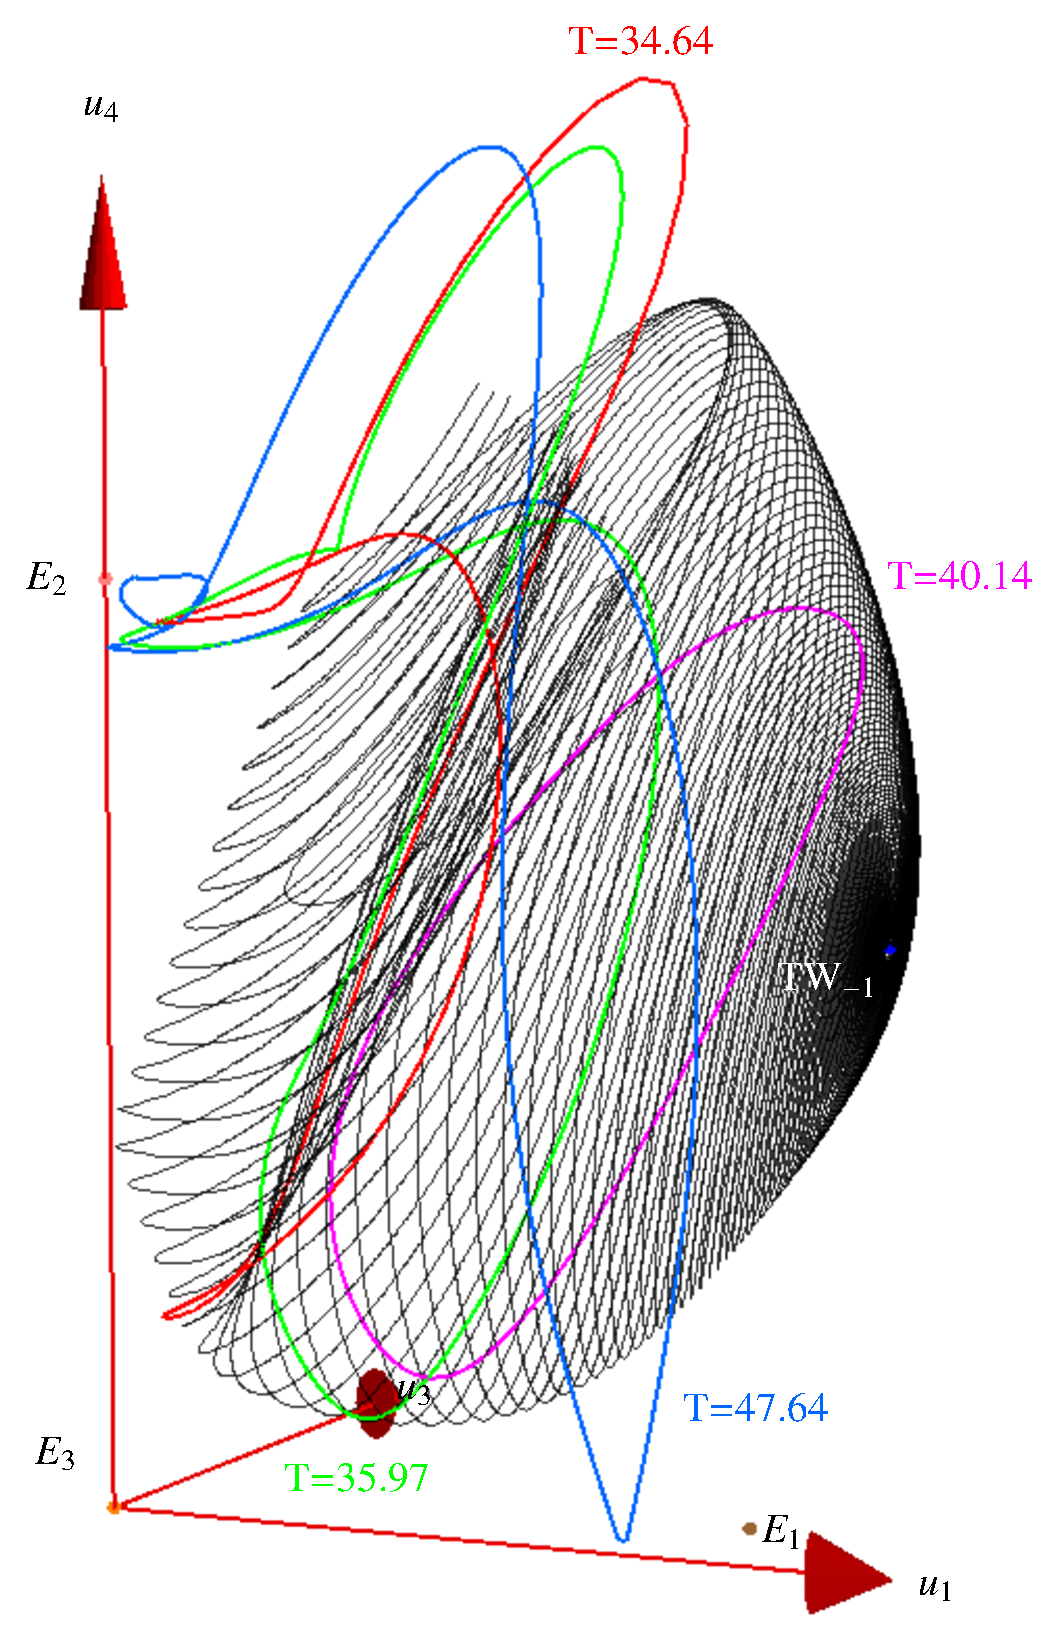
\includegraphics[width=0.45\textwidth, clip=true]{../figs/ks22tw1umInv2}
~(\textit{b})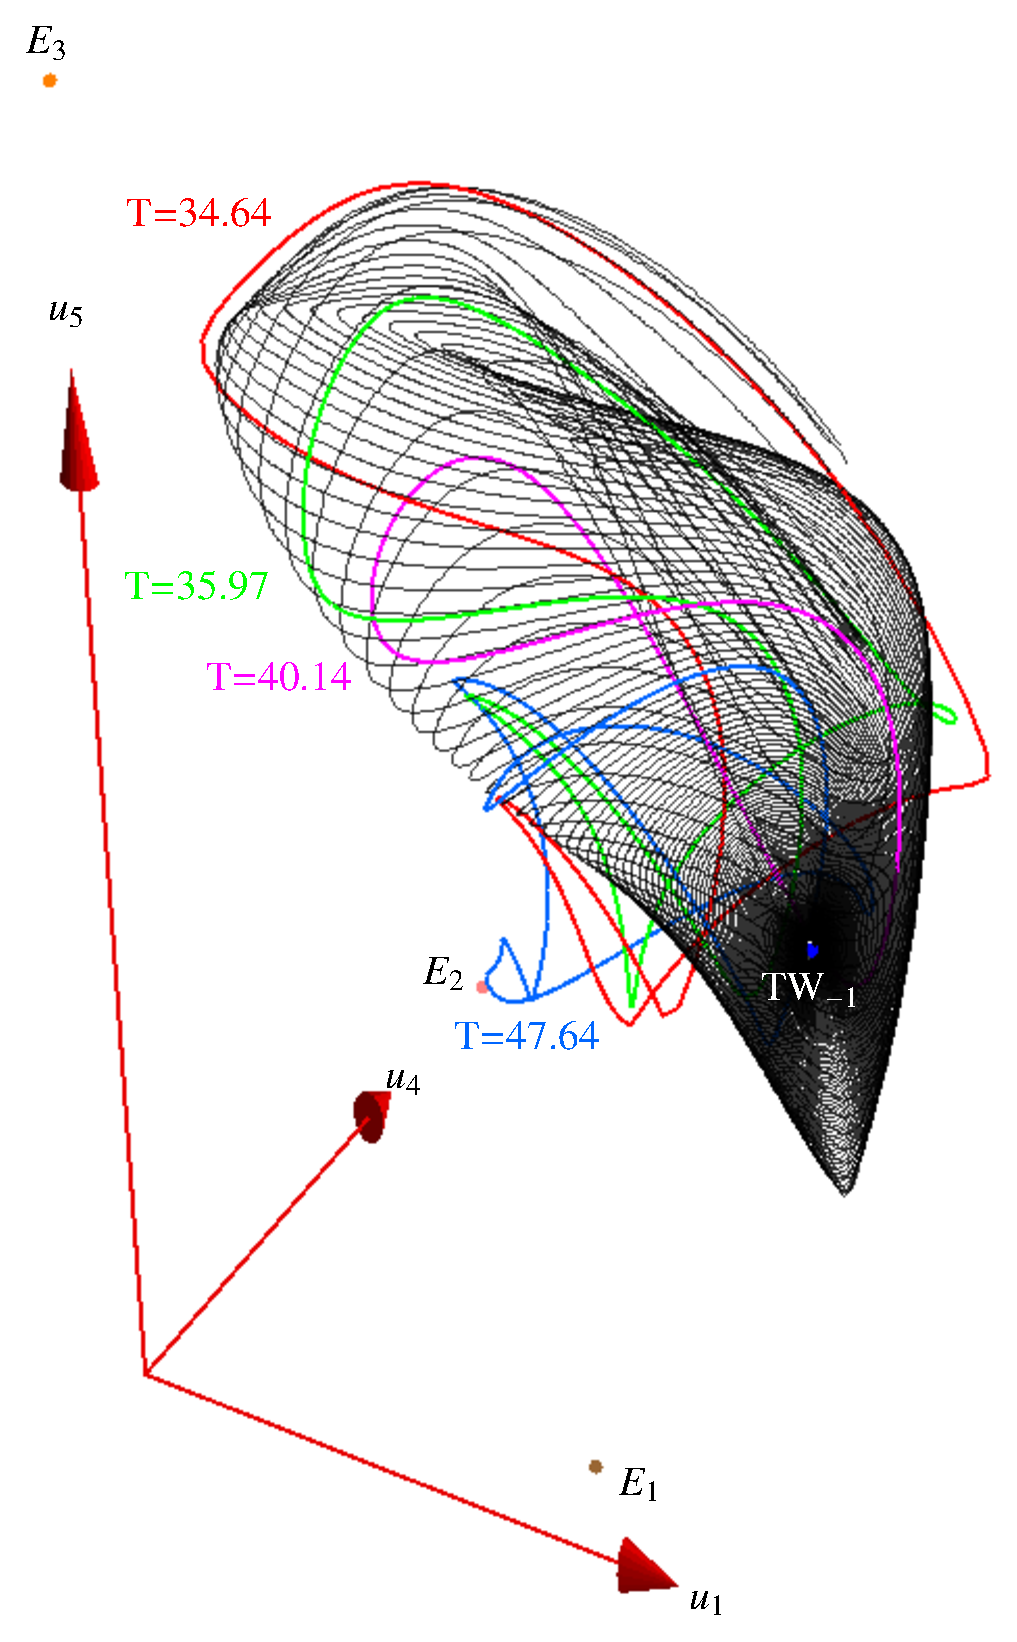
\includegraphics[width=0.45\textwidth, clip= true]{../figs/ks22tw1umInv}
\end{center}
\caption[\KS\ \SOn{2} reduced \statesp\ projection, $\REQV{-}{1}$ unstable manifold]
{Two different projections of L=22 \KS\ dynamics on invariants
given in \reftab{tab:SO2n6modif}. We plot a few selected {\rpo s} and part of
the unstable manifold of
$\REQV{-}{1}$ in black, with trajectories originating along the eigenspace
corresponding to \eigExp[1].}
\label{fig:TW1red}
\end{figure}
%%%%%%%%%%%%%%%%%%%%%%%%%%%%%%%%%%%%%%%%%%%%%%%%%%%%%%%%%%%%%%%%

%%%%%%%%%%%%%%%%%%%%%%%%%%%%%%%%%%%%%%%%%%%%%%%%%%%%%%%%%%%%%%%%%%
\begin{figure}[t]
\begin{center}
  (\textit{a})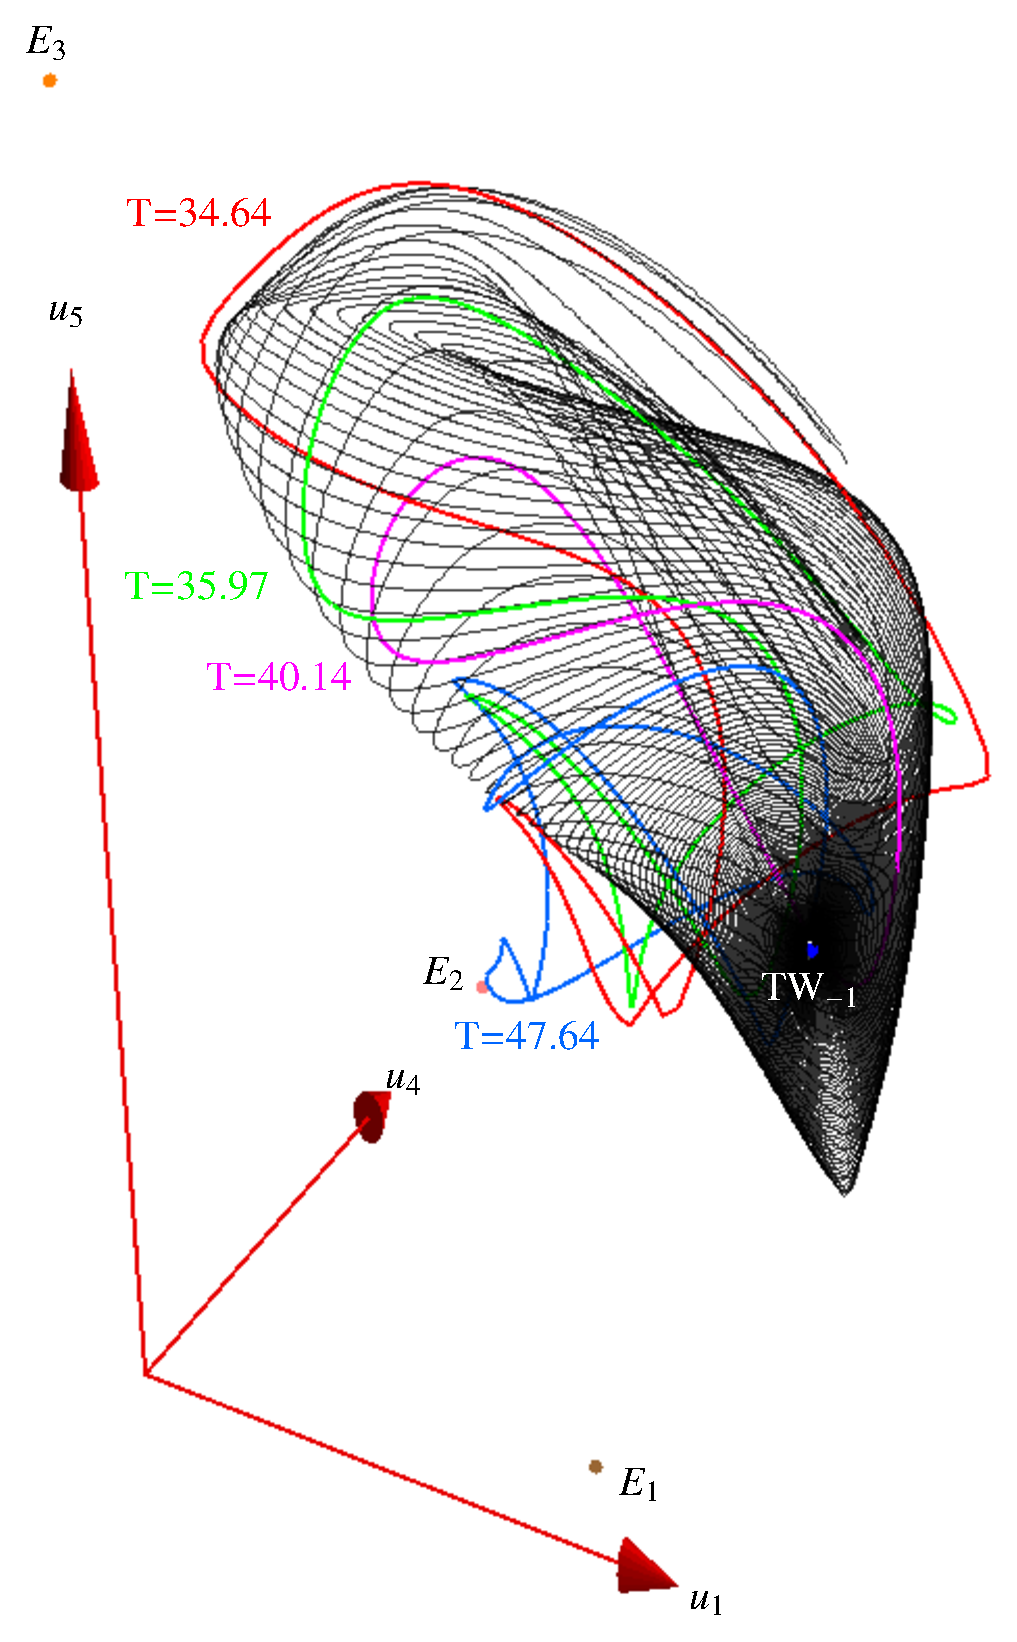
\includegraphics[width=0.45\textwidth, clip=true]{../figs/ks22tw1umInv}
~(\textit{b})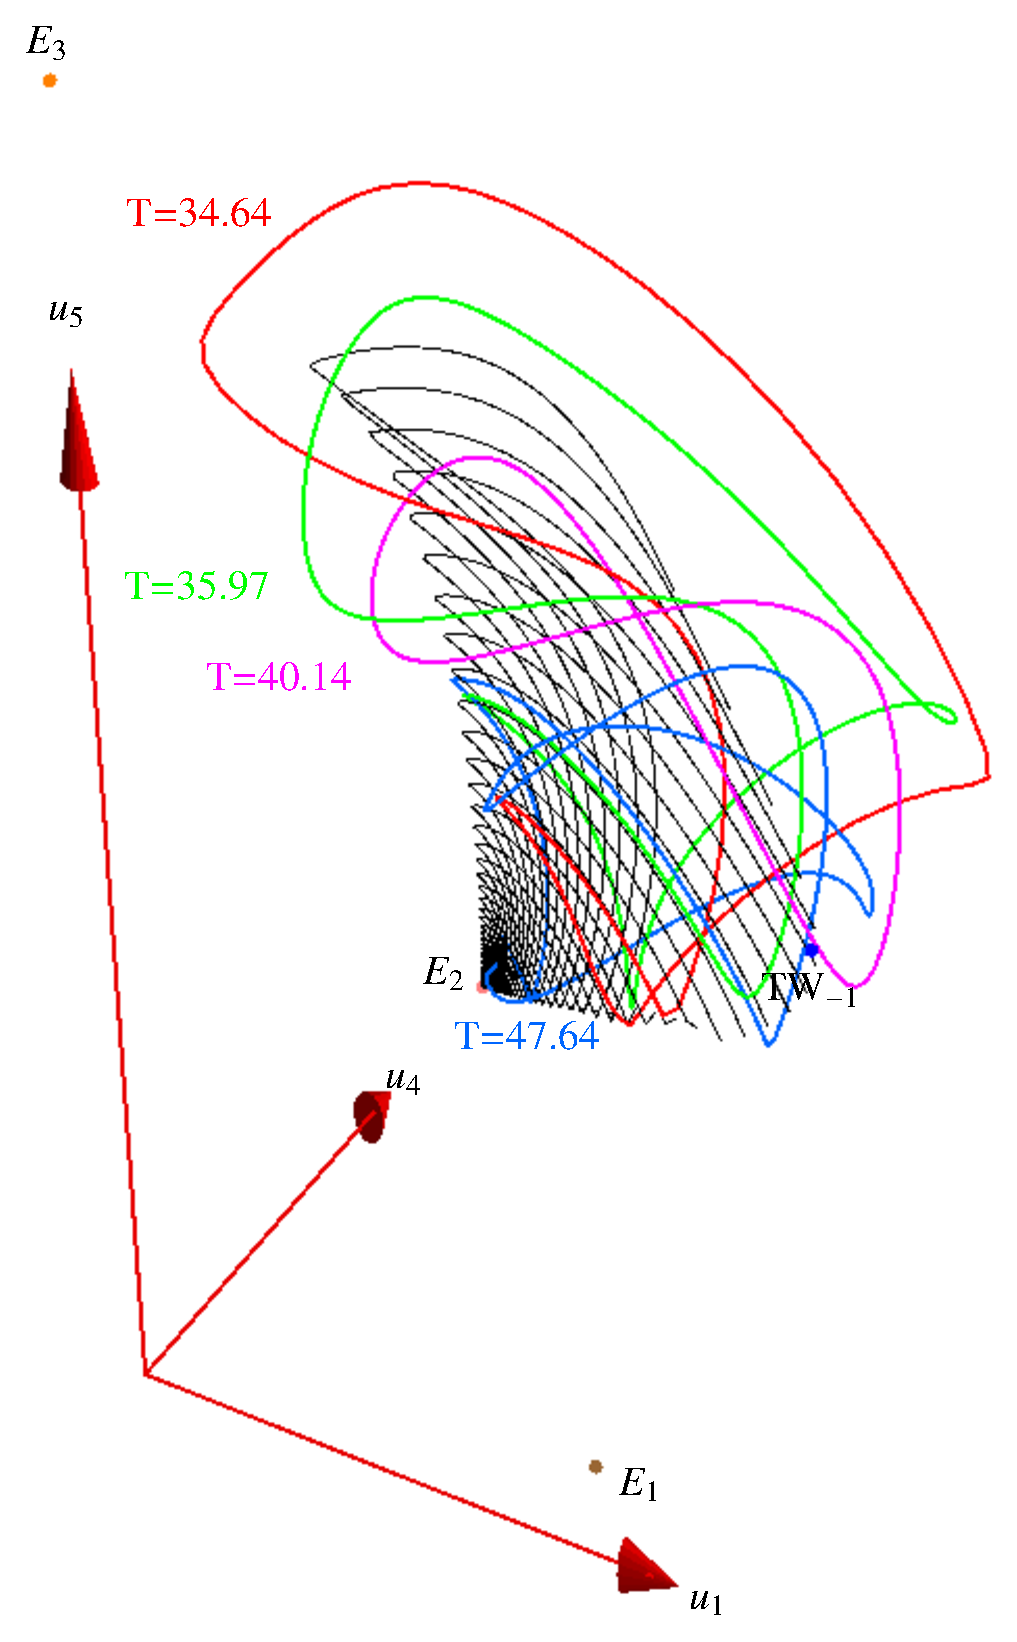
\includegraphics[width=0.45\textwidth, clip= true]{../figs/ks22-2wUMInv}
\end{center}
\caption[\KS\ \SOn{2} reduced \statesp\ projection, $\REQV{-}{1}$ and $\EQV{1}$ unstable manifolds]
{Two different projections of L=22 \KS\ dynamics on invariants
given in \reftab{tab:SO2n6modif}. We plot a few selected {\rpo s} and  (\textit{a}) part of
the unstable manifold of
$\REQV{-}{1}$ in black, with trajectories originating along the eigenspace
corresponding to \eigExp[1],  (\textit{b}) part of the unstable manifold of \EQV{1}, in black.}
\label{fig:TW1-E2red}
\end{figure}
%%%%%%%%%%%%%%%%%%%%%%%%%%%%%%%%%%%%%%%%%%%%%%%%%%%%%%%%%%%%%%%%
